\begin{figure}[h!]
    \centering
    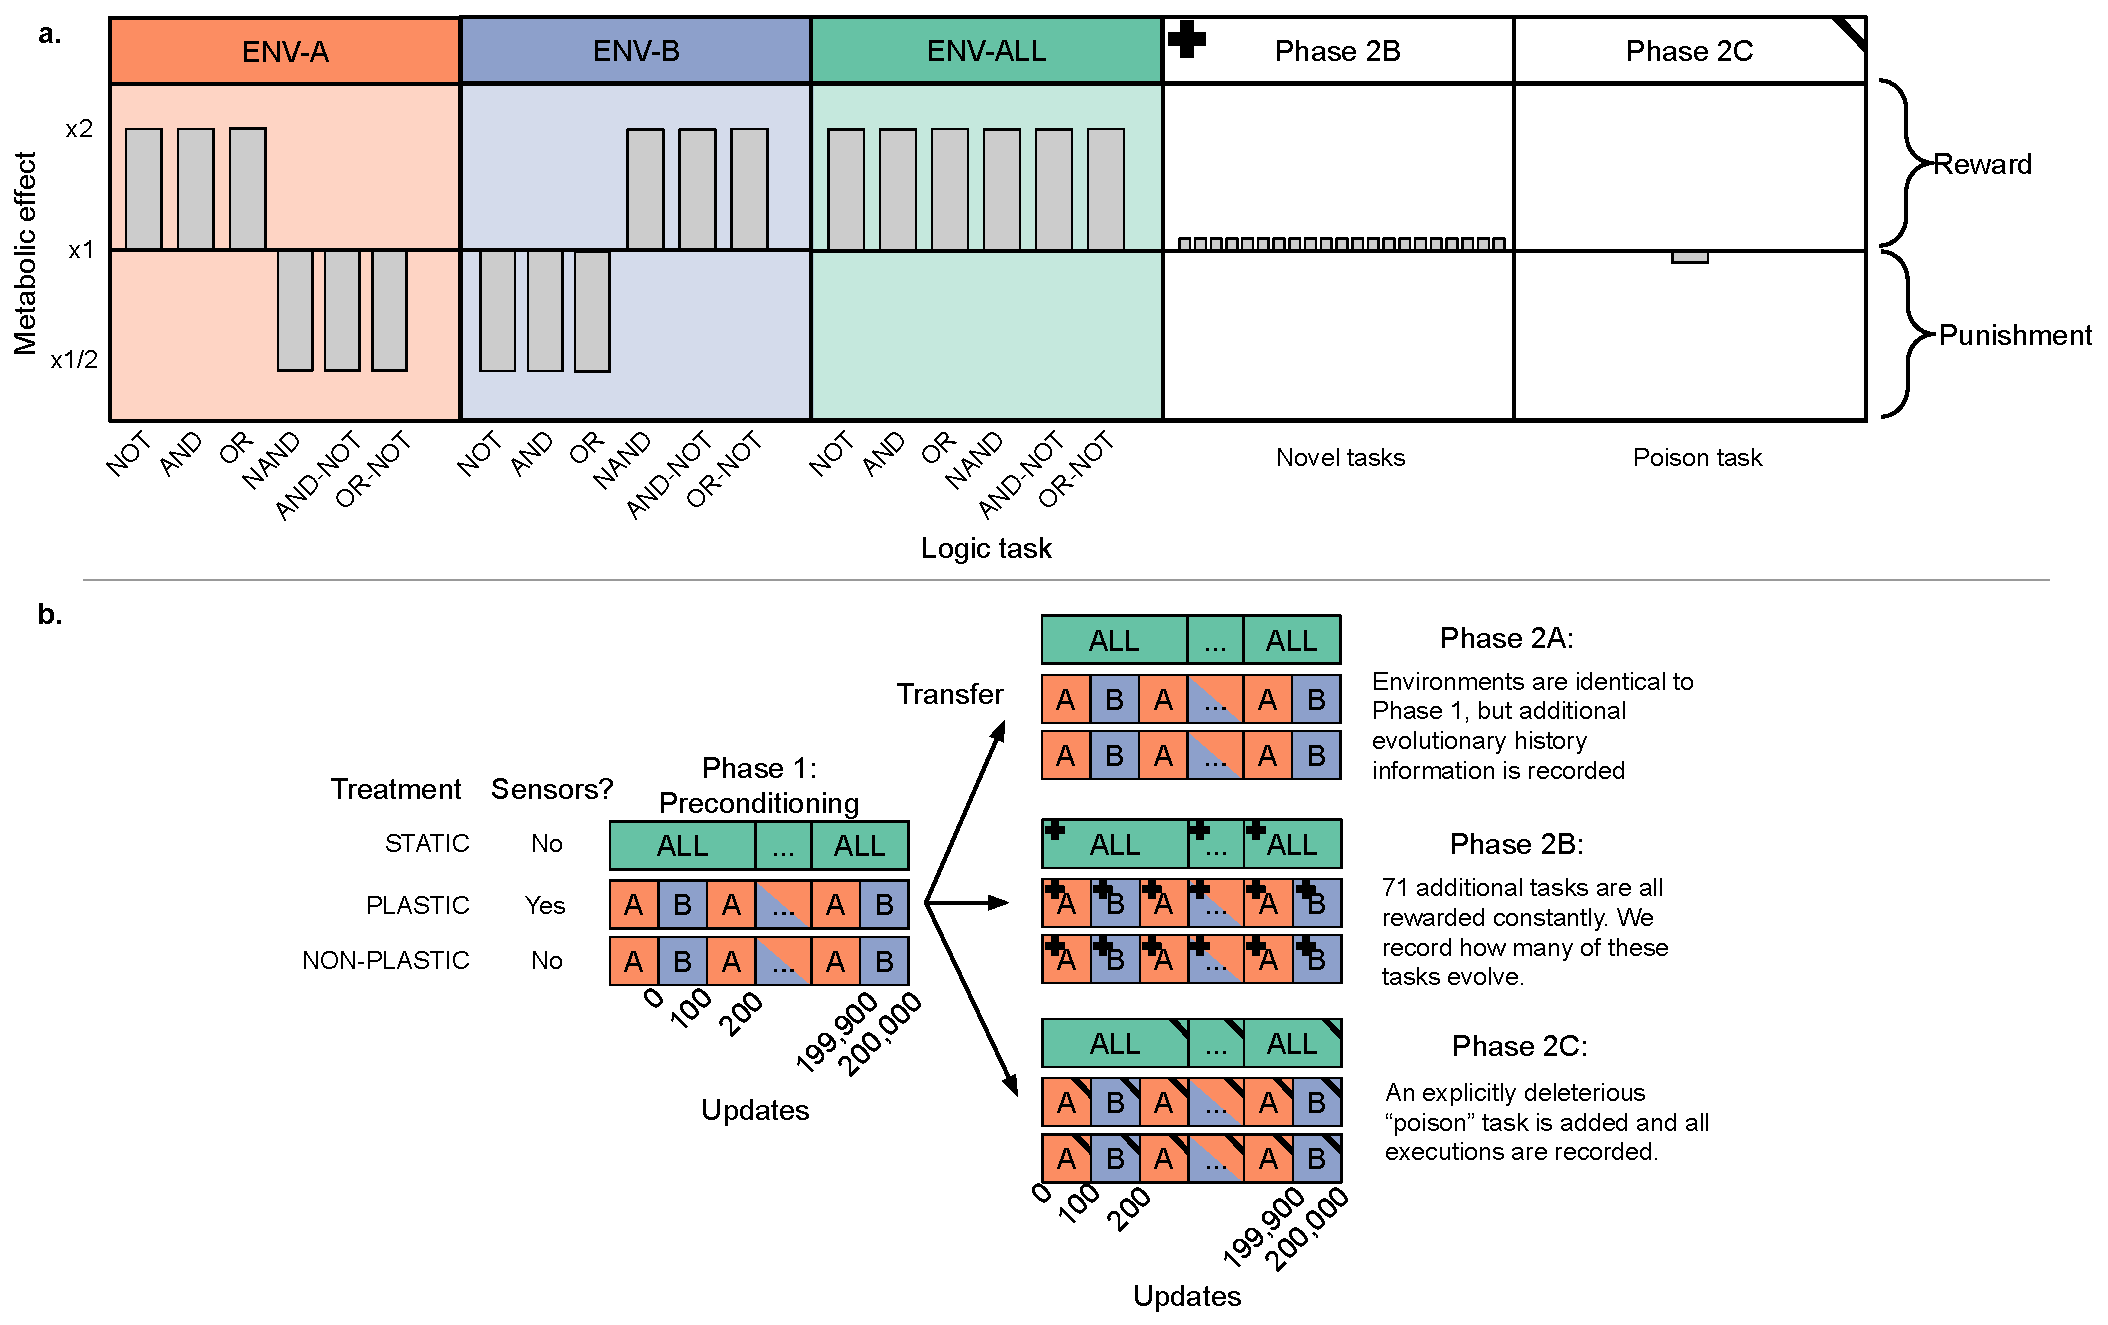
\includegraphics[width=1\textwidth]{media/experimental-design.pdf}
    \caption{\small
    \textbf{Overview of experimental design.}
    The first three plots in panel (a) show the environments used in every experiment and whether they reward or punish each base task. 
    Additionally, the last two subplots in (a) show the additional tasks added in phases 2B and 2C. 
    All novel tasks in phase 2B confer a 10\% metabolic reward, while executing the poisonous task in phase 2C causes a 10\% metabolic punishment (bars not drawn to scale). 
    Panel (b) shows treatment differences and experimental phases. 
    Treatments are listed on the left, with each treatment specifying its environmental configuration and whether sensors are functional.
    % consisting of an environment timeline and whether sensors are functional. 
    % This also shows Phase 1, the preconditioning phase.  
    We conducted three independent two-phase experiments, each described on the right.
    % We conducted experiments using three different second phases, as shown on the right. 
    Phases 2B and 2C are textured to match their task definitions in panel (a). 
    Phase one is repeated for \textit{each} experiment with 100 replicate populations per treatment per experiment. 
    For each replicate at the end of phase one, we used an organism of the most abundant genotype to found the second phase population. 
    All STATIC and NON-PLASTIC populations move on to phase two, but PLASTIC populations only continue to the second phase if their most abundant genotype exhibits optimal plasticity. 
    Metrics are recorded only in phase two.
    }
    \label{fig:experimental-design}
\end{figure}